\documentclass{article}
\usepackage{amsmath,amsfonts}
\usepackage[toc]{appendix}
\usepackage{array}
\usepackage{bm}
\usepackage{cancel}
\usepackage[labelfont=bf]{caption}
\usepackage[usenames, dvipsnames]{color}
\usepackage{empheq}
\usepackage{float}
\usepackage[most]{tcolorbox}
\usepackage{enumerate}
\usepackage{graphicx}
\usepackage{tabularx}
\usepackage{textcomp}
\usepackage{tikz}
\usetikzlibrary{calc}
\usetikzlibrary{math}
\usepackage{url}
\usepackage{verbatim}
\usepackage{xcolor}
\usepackage{wasysym}
\definecolor{linkborder}{RGB}{204,229,255}
\usepackage{hyperref}\hypersetup{linkbordercolor=linkborder}

\definecolor{vanish}{RGB}{224,224,224}
\renewcommand{\arraystretch}{2}

\newtcbox{\boxEq}[1][]{
    nobeforeafter, tcbox raise base,
    colframe=black!30!black,
    colback=white!30, boxrule=0.4pt,
    sharp corners}
\numberwithin{equation}{section}

\begin{document}
    \begin{titlepage}
        \centering
        \vspace*{\fill}  % Pushes content to vertical center

        {\Huge\bfseries Modelling of Diffuse Scattering Effects for Outdoor Ray Tracing \par}
        \vspace{1cm}
        
        {\Large Andrew Whelan \par}
        \vspace{0.5cm}
        
        {\large \date{\today} \par}

        \vspace*{\fill}  % Pushes remaining space below
    \end{titlepage}

    \thispagestyle{empty}
    \setcounter{page}{0}
    \tableofcontents

    \newpage
    \small
    \section*{Notation}
        \addcontentsline{toc}{section}{Notation}
        \subsection*{Mathematical}
            \begin{tabular}{ m{6em} m{30em} m{0em} }
                \( \partial_t \) & \( \displaystyle \frac{\partial}{\partial t}\) & \\
                \( j \) & Imaginary unit ( \( j^2 = -1 \) ) & \\
                \(R_{x, \theta},R_{y, \theta},R_{z, \theta} \) & \( \displaystyle 
                    \begin{pmatrix} 
                        1 & 0 & 0 \\
                        0 & \cos \theta & -\sin \theta \\ 
                        0 & \sin \theta & \cos \theta 
                    \end{pmatrix} 
                    \), \( \displaystyle 
                    \begin{pmatrix} 
                        \cos \theta & 0 & \sin \theta \\ 
                        0 & 1 & 0 \\ 
                        - \sin \theta & 0 & \cos \theta 
                    \end{pmatrix}
                    \), \( \displaystyle
                    \begin{pmatrix} 
                        \cos \theta & -\sin \theta & 0 \\ 
                        \sin \theta & \cos \theta & 0 \\ 
                        0 & 0 & 1 
                    \end{pmatrix} 
                    \) \\
                \(P_{xz}\) & \( \displaystyle 
                    \begin{pmatrix} 
                        0 & \hspace{2em} 0 & \hspace{2em} 1 \\ 
                        0 & \hspace{2em} 1 & \hspace{2em} 0 \\ 
                        1 & \hspace{2em} 0 & \hspace{2em} 0 
                    \end{pmatrix} 
                    \)
            \end{tabular}
        \subsection*{Microscopic Fields}
            \begin{tabular}{ m{7em} m{24em} m{4em} }
                \( E \) & Electric Field Intensity & [V m\textsuperscript{-1}] \\
                \( H \) & Magnetic Field Intensity & [A m\textsuperscript{-1}] \\
            \end{tabular}
        \subsection*{Macroscopic Fields}
            \begin{tabular}{ m{7em} m{24em} m{4em} }
                \( D \) & Electric Flux Density & [C m\textsuperscript{-2}] \\
                \( B \) & Magnetic Flux Density & [Wb m\textsuperscript{-2}] \\
            \end{tabular}
        \subsection*{Field Sources}
            \begin{tabular}{ m{7em} m{24em} m{4em} }
                \( \displaystyle J_{c/d/i} \) & Electric Current Density 
                    \textsubscript{(conduction/displacement/impressed)} &
                    [A m\textsuperscript{-2}] \\
                \( \displaystyle \mathfrak{M}_{d/i} \) & Magnetic Current Density 
                    \textsubscript{(displacement/impressed)} & [V m\textsuperscript{-2}]
                    \\
                \( \displaystyle \rho_{e} \) & Electric Charge Density & 
                    [C m\textsuperscript{-2}] \\
                \( \displaystyle \rho_{m} \) & Magnetic Charge Density & 
                [Wb m\textsuperscript{-2}]
            \end{tabular}
        \subsection*{Constitutive Parameters}
            \begin{tabular}{ m{7em} m{24em} m{4em} }
                \( \displaystyle \epsilon \) & Permittivity & [F m\textsuperscript{-1}] \\
                \( \displaystyle \mu \) & Permeability & [H m\textsuperscript{-1}] \\
                \( \displaystyle \sigma \) & Conductivity & [S m\textsuperscript{-1}] \\
            \end{tabular}
        \subsection*{Waves}
            \begin{tabular}{ m{7em} m{24em} m{4em} }
                \( \displaystyle f \) & Frequency & [s\textsuperscript{-1}] \\
                \( \displaystyle k \)\textsuperscript{\eqref{eq:wavenumber}} &
                    Wavenumber & [m\textsuperscript{-1}]  \\
                \( \displaystyle \alpha \)\textsuperscript{\eqref{eq:attenuationConstant}}
                    & Wave Attenuation & [m\textsuperscript{-1}]  \\
                \( \displaystyle \lambda := \frac{2 \pi}{k} \) & Wavelength & [m] \\
                \( \displaystyle \omega := 2 \pi f \) & Angular Frequency &
                    [s\textsuperscript{-1}] \\
                \( \displaystyle \eta := \sqrt{\frac{j \omega \mu}{\sigma + j \omega
                    \epsilon}} \) &
                    Intrinsic Impedance & [S\textsuperscript{-1}] \\
                \( \displaystyle v_g := \partial_k \omega \) & Group velocity of wave
                    (envelope velocity) & [ms\textsuperscript{-1}]  \\
                \( \displaystyle v_p := \frac{\omega}{k} \) & Phase velocity of wave
                    (peak/trough velocity) & [ms\textsuperscript{-1}]  \\
            \end{tabular}
            \normalsize
    \newpage
    \section{Effective Roughness Model}
        This model is a modification of Geometrical Optics in which, in addition to the
        specular component, each point impinging on the middle of a surface element $dW$
        gives a diffuse contribution $dE_d$ to the scattered field $E_s$ whose amplitude $\left|
        dE_d \right|$ is given by
        \begin{equation} \label{eq:scatteringAmpER}
           \left| dE_d \right| \propto \sqrt{\frac{dW \cos \theta_i \cos \theta_s}{\pi}}
           \frac{1}{r_i r_s}
        \end{equation}
        with the constant of proportionality depending on the incident amplitude and a
        scattering parameter $S$. Specifically, we have
        \begin{subequations}
            \begin{align}
                \left| dE_d \right| &= S \Upsilon \sqrt{dW}, \quad \text{where} \\
                \Upsilon &= \sqrt{\frac{60 G_t P_t \cos \theta_i \cos \theta_s}{\pi}}
                \frac{1}{r_i r_s}
            \end{align}
        \end{subequations}
        \subsection{Uniform Plane Wave Incident on PEC}    
            We start with a setup as per Figure~\ref{fig:planeWavePEC}.
            \vspace*{\fill}
            \begin{figure}[H] 
            \begin{center}
            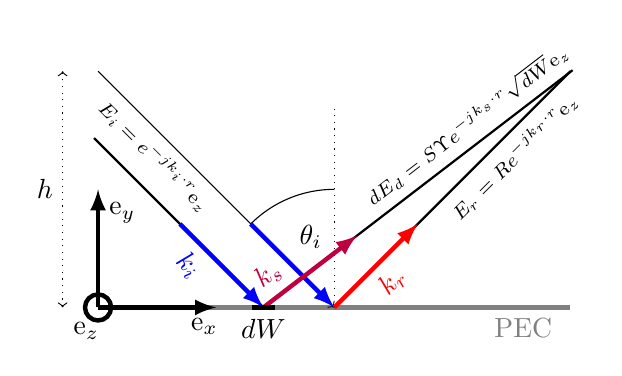
\begin{tikzpicture}[scale=1.5]
            \newcommand{\drawLabelledArrow}[9]{%
                \tikzmath{
                    \xArrowStart = #1; 
                    \yArrowStart = #2;
                    \arrowLen = #3; 
                    \arrowAngle = #4;
                    \labelAngleShift = #7;
                    \xArrowEnd = \xArrowStart + \arrowLen * cos(\arrowAngle);
                    \yArrowEnd = \yArrowStart + \arrowLen * sin(\arrowAngle);
                }
                % Define the text and color as regular TeX macros
                \def\arrowLabel{#5}%
                \def\arrowColor{#6}%
                \def\arrowStyle{#8}
                \def\labelStyle{#9}
                % Draw
                \draw[#8, \arrowColor] 
                    (\xArrowStart, \yArrowStart) -- (\xArrowEnd, \yArrowEnd)
                    node[#9, rotate=\arrowAngle+\labelAngleShift]
                        {\arrowLabel};
            }
            % Call the macro with: xStart, yStart, length, angle, label, label offset, color
            % Wall
            \tikzmath{
                    \xObstacleStart = 0;            
                    \yObstacleStart = 0;            
                    \obstacleLen = 4;               
                    \obstacleAngle = 0;            
                    \xObstacleCentre = 0.5*\obstacleLen*cos(\obstacleAngle);
                    \yObstacleCentre = 0.5*\obstacleLen*sin(\obstacleAngle);
            }
            \def\obstacleLabel{PEC}
            \def\obstacleColor{gray}
            \def\obstacleArrowStyle{ultra thick}
            \drawLabelledArrow{\xObstacleStart}{\yObstacleStart}{\obstacleLen}{\obstacleAngle}
                {\obstacleLabel}{\obstacleColor}{0}{\obstacleArrowStyle}{pos=0.9,below}
            % Incident Ray
            \tikzmath{
                    \xIncidentStart = \xObstacleStart + \xObstacleCentre);
                    \yIncidentStart = \yObstacleStart + \yObstacleCentre);
                    \incidentAngle = \obstacleAngle + 135;
                    \incidentLen = \obstacleLen/(abs(2*cos(\incidentAngle)));%\obstacleLen * ; 
            }
            \def\incidentLabel{\begingroup \scriptsize $E_i = e^{-jk_i \cdot r} \text{e}_z$ \endgroup}%= E_0 e^{-jk_i \cdot r} \text{e}_z$}
            \def\incidentColor{black}
            \def\incidentArrowStyle{<-}
            \drawLabelledArrow{\xIncidentStart}{\yIncidentStart}{\incidentLen}{\incidentAngle}
                {\incidentLabel}{\incidentColor}{180}{\incidentArrowStyle}{pos=0.7,below}

            % Normal Ray
            \tikzmath{
                    \normalLen = \obstacleLen*(0.4); 
                    \xNormalStart = (\normalLen/2)*sin(\obstacleAngle) + \xObstacleStart +
                        \xObstacleCentre;
                    \yNormalStart = 0.9 -(\normalLen/2)*cos(\obstacleAngle) + \yObstacleStart +
                        \yObstacleCentre;
                    \normalAngle = \obstacleAngle + 90;
            }
            \def\normalLabel{}
            \def\normalColor{black}
            \def\normalArrowStyle{thick}
            \drawLabelledArrow{\xNormalStart}{\yNormalStart}{\normalLen}{\normalAngle}
                {\normalLabel}{\normalColor}{180}{dotted}{midway,below}
            
            \pgfmathsetmacro\xFudge{\xObstacleCentre - sin(\obstacleAngle)}
            \pgfmathsetmacro\yFudge{\yObstacleCentre + cos(\obstacleAngle)}
            \draw (\xFudge, \yFudge) arc (\obstacleAngle+90:\obstacleAngle+135:1);
            \tikzmath{
                \xIncidentE = \xIncidentStart + \incidentLen * cos(\incidentAngle);
                \yIncidentE = \yIncidentStart + \incidentLen * sin(\incidentAngle);
            }
            \node[draw, circle, ultra thick] (A) at (\xObstacleStart, \yObstacleStart)
                {};
            \node at (-0.1,-0.2) {$\text{e}_z$};
            \drawLabelledArrow{\xObstacleStart}{\yObstacleStart}{1.0}{0}
                {$\text{e}_x$}{\normalColor}{0}{-{latex}, ultra thick}{pos=0.9,below}
            \drawLabelledArrow{\xObstacleStart}{\yObstacleStart}{1.0}{90}
                {$\text{e}_y$}{\normalColor}{270}{-{latex}, ultra thick}{pos=0.8,right}
            \node at (1.8,0.6) {$\theta_i$};
            \tikzmath{
                \txHeight = \incidentLen * sin(\incidentAngle);
                \heightStart = \xObstacleStart - 0.3;
            }
            \drawLabelledArrow{\heightStart}{\yObstacleStart}{\txHeight}{90}
                {$h$}{\normalColor}{270}{<->, dotted}{pos=0.5,left}
            \tikzmath{
                \waveVectorAngle = 180- \incidentAngle;
            }
            \drawLabelledArrow{\xIncidentStart}{\yIncidentStart}{1}
                {\incidentAngle}{}{blue}{180}{{latex}-, ultra thick}{pos=1.0,below}
            %\draw (\xFudge, \yFudge) arc
            %    (\obstacleAngle+90:\obstacleAngle+\waveVectorAngle:1);
            %\node at (2.2,0.5) {$\theta_i$};
            \drawLabelledArrow{\xIncidentStart}{\yIncidentStart}{\incidentLen}
                {\waveVectorAngle}{\begingroup \scriptsize $E_r = Re^{-jk_r \cdot
                r}\text{e}_z $\endgroup}{black}{0}{thick}{pos=0.7,below}
            \drawLabelledArrow{\xIncidentStart}{\yIncidentStart}{1}
                {\waveVectorAngle}{$k_{r}$}{red}{0}{-{latex}, ultra thick}{pos=0.5,below}
            \tikzmath{
                \xNonCoherentRay = \xIncidentStart - 0.6;
                \nonCoherentRayLen = \incidentLen - 0.8;%( \incidentLen - 0.5 ) / cos( 180 - \incidentAngle );
                \nonCoherentRayAngle = \incidentAngle;
            }
            \drawLabelledArrow{\xNonCoherentRay}{\yIncidentStart}{\nonCoherentRayLen}
                {\nonCoherentRayAngle}{}{black}{0}{thick}{pos=0.7,above}
            \drawLabelledArrow{\xNonCoherentRay}{\yIncidentStart}{1}
                {\nonCoherentRayAngle}{$k_i$}{blue}{180}{{latex}-,ultra thick}{pos=0.7,below}
            \drawLabelledArrow{\xNonCoherentRay}{\yIncidentStart}{3.3}
                {37.5}{\begingroup \scriptsize $dE_d = S\Upsilon e^{-jk_s \cdot r} \sqrt{dW} \text{e}_z$ \endgroup}{black}{0}{thick}{pos=0.7,above}
            \drawLabelledArrow{\xNonCoherentRay}{\yIncidentStart}{1}
                {37.5}{$k_{s}$}{purple}{0}{-{latex},ultra thick}{pos=0.2,above}
            \tikzmath{
                \xSurfaceElement = \xNonCoherentRay - 0.1;
                \surfaceElementLen = 0.2;
            }
            \drawLabelledArrow{\xSurfaceElement}{\yIncidentStart}{\surfaceElementLen}
                {0}{$dW$}{black}{0}{ultra thick}{pos=0.5,below}
            \end{tikzpicture}
            \caption{A uniform plane wave strikes a PEC. The overall scattered wave is $E_s = E_r + E_d$. $E_r$ is just the usual specular component of geometrical optics, multiplied by $R$, a roughness parameter. $E_d$ is the diffuse component, which will be a sum/integral of contributions along the wall, one of which is shown here, for a drawn surface element $dW$}
            \label{fig:planeWavePEC}
            \end{center}
            \end{figure}

    \newpage
    \renewcommand{\thesubsection}{\Alph{subsection}}
    \numberwithin{equation}{subsection}
    \appendix
    \section*{Appendices}
    \addcontentsline{toc}{section}{Appendices}
    \subsection{Mathematical Identities and Theorems}
        \begin{subequations} \label{eq:integralVectorTheorems}
            \begin{align}
                \oint_C A \cdot dl &= \iint_S (\nabla \times A) \cdot ds
                    \label{eq:stokes} \\
                \oiint_S A \cdot ds &= \iiint_V (\nabla \cdot A) dv \label{eq:divergence}
            \end{align}
        \end{subequations}
        \begin{subequations} \label{eq:vectorDifferentialIdentities}
            \begin{align}
                \nabla \cdot (A \times B) &= B \cdot (\nabla \times A) - A \cdot (\nabla
                    \times B) \label{eq:divOfCurlOfProduct}
            \end{align}
        \end{subequations}
        \newpage
    \subsection{Maxwell's Equations}
        \subsubsection{Differential Form}
            \begin{subequations}\label{eq:Maxwell}
                \begin{align}
                    \nabla \times E &= - \partial_t B \begingroup \textcolor{vanish}{
                        - \mathfrak{M}_i } \endgroup \label{eq:MaxwellFaraday} \\
                    \nabla \times H &= \ \ \partial_t D + J_{c} + J_{i} 
                        \label{eq:AmpereMaxwell} \\
                    \nabla \cdot D &= \ \ \rho_e \label{eq:GaussElectric} \\
                    \nabla \cdot B &= \ \ 0 \begingroup \textcolor{vanish}{
                        \quad = \rho_m} \endgroup \label{eq:GaussMagnetic}
                \end{align}
            \end{subequations}
        \subsubsection{Constitutive Relations} 
            The material properties of a medium can be modelled without specifying 
            microscopic structure:
            \begin{subequations}\label{eq:Constitutive}
                \begin{align}
                    D &= \epsilon E \label{eq:ConstitutiveElectric} \\ 
                    B &= \mu H \label{eq:ConstitutiveMagnetic} \\
                    J_c &= \sigma E \label{eq:ConstitutiveCurrentDensity}
                \end{align}
            \end{subequations}
        \subsubsection{Integral Form}
            The below can be derived from taking the surface integral of the curl
            equations, the volume integral of the divergence equations, and applying 
            \eqref{eq:integralVectorTheorems}:
            \begin{subequations}\label{eq:MaxwellIntegral}
                \begin{align}
                    \oint_C E \cdot dl &=  - \partial_t \iint_S B \cdot ds \begingroup 
                        \textcolor{vanish}{- \iint_S \mathfrak{M_i} \cdot ds} \endgroup 
                        \label{eq:MaxwellFaradayIntegral} \\
                    \oint_C H \cdot dl &= \partial_t \iint_S D \cdot ds + \iint_S 
                        ( J_c + J_i ) \cdot ds \label{eq:AmpereMaxwellIntegral} \\
                    \oiint_S D \cdot ds &= \iiint_V \rho_e \cdot dv 
                        \label{eq:GaussElectricIntegral} \\
                    \oiint_S B \cdot ds &= 0 \begingroup \textcolor{vanish}{= \iiint_V 
                        \rho_m \cdot dv} \endgroup \label{eq:GaussMagneticIntegral}
                \end{align}
            \end{subequations}
        \subsubsection{Uncoupled Form}
            \begin{subequations} \label{eq:fieldEqs}
                \begin{align}
                    (\mu \epsilon \partial^2_t + \mu \sigma \partial_t - \nabla^2 ) E &
                        \begingroup \textcolor{vanish}{+ \nabla \times \mathfrak{M}_i} 
                        \endgroup + \mu \partial_t J_i + \frac{1}{\epsilon} \nabla
                        \rho_e = 0 \label{eq:electricFieldEq} \\
                    (\mu \epsilon \partial^2_t + \mu \sigma \partial_t - \nabla^2 ) H & -
                        \nabla \times J_i \begingroup \textcolor{vanish}{+ \epsilon
                        \partial_t \mathfrak{M}_i + \frac{1}{\mu} \nabla \rho_m + \sigma
                        \mathfrak{M}_i} \endgroup = 0 \label{eq:magneticFieldEq}
                \end{align}
            \end{subequations}
        \subsubsection{Time-Harmonic Form}
            To obtain solutions we usually look at time-harmonic solutions, and can then
            use Fourier series to express other forms in terms of these. The time
            harmonic forms of \eqref{eq:fieldEqs} are obtained by replacements
            $\partial_t \to \omega j$, $\partial_t^2 \to - \omega^2$:
            \begin{subequations} \label{eq:fieldEqsTH}
                \begin{align}
                    (- \mu \epsilon \omega^2 + \mu \sigma \omega j - \nabla^2 ) E &
                        \begingroup \textcolor{vanish}{+ \nabla \times \mathfrak{M}_i}
                        \endgroup + \mu \omega j J_i + \frac{1}{\epsilon} \nabla \rho_e
                        = 0 \label{eq:electricFieldEqTH} \\
                    (-\mu \epsilon \omega^2 + \mu \sigma \omega j - \nabla^2 ) H & -
                        \nabla \times J_i \begingroup \textcolor{vanish}{+ \epsilon
                        \omega j \mathfrak{M}_i + \frac{1}{\mu} \nabla \rho_m + \sigma
                        \mathfrak{M}_i} \endgroup = 0 \label{eq:magneticFieldEqTH}
                \end{align}
            \end{subequations}

            Note that the quantity $- \mu \epsilon \omega^2 + \mu \sigma \omega j $ can be
            expressed as the square of a single complex number $\gamma = \alpha + kj$.
            Solving for $\alpha$ and $k$, we get
            \begin{subequations}
            \begin{align} \label{eq:attenuationConstant}
                \alpha &= \omega \sqrt{\mu \epsilon} \left( \frac{1}{2} \left( \sqrt{1 +
                    \left( \frac{\sigma}{\omega \epsilon} \right)^2 } - 1 \right)
                    \right)^{\frac{1}{2}} \\
                k &= \omega \sqrt{\mu \epsilon} \left( \frac{1}{2} \left( \sqrt{1 + \left(
                    \frac{\sigma}{\omega \epsilon} \right)^2 } + 1 \right)
                    \right)^{\frac{1}{2}} \label{eq:wavenumber}
            \end{align}
            \end{subequations}
        \subsubsection{Source-Free Time Harmonic Equations}
            The source-free ($\rho_e = \rho_m = J_i = \mathfrak{M}_i = 0$) versions of
            \eqref{eq:fieldEqsTH} are
            \begin{subequations} \label{eq:fieldEqsSF}
                \begin{align}
                    (- \mu \epsilon \omega^2 + \mu \sigma \omega j - \nabla^2 ) E & = 0
                        \label{eq:electricFieldEqSF} \\
                    ( - \mu \epsilon \omega^2 + \mu \sigma \omega j - \nabla^2 ) H & = 0
                        \label{eq:magneticFieldEqSF}
                \end{align}
            \end{subequations}
        \subsubsection{Boundary Conditions}
            \scriptsize
            \begin{tabular}{ | m{6.5em} || m{7.9em} | m{7.5em} | m{7.7em} | m{7.9em} | }
                \hline
                    & \textbf{General} & \textbf{Finite \( \sigma \), no source/charge} &
                    \textbf{Medium 1 PEC} & \textbf{Medium 1 PMC} \\
                \hline\hline
                    \( E_{\parallel} := n \times E \) & \( E_{\parallel 2} -
                    E_{\parallel 1} = -\mathfrak{M}_s \) & \( E_{\parallel 2} -
                    E_{\parallel 1} = 0 \) & \(E_{\parallel 2} = 0 \) & \( E_{\parallel
                    2} = -\mathfrak{M}_s \) \\
                \( H_{\parallel} := n \times H \) & \( H_{\parallel 2} - H_{\parallel 1} =
                    J_s \) & \( H_{\parallel 2} - H_{\parallel 1} = 0 \) & \( H_{\parallel
                    2} = J_s \) & \( H_{\parallel 2} = 0 \) \\
                \( D_{\perp} := n \cdot D \) & \( D_{\perp 2} - D_{\perp 1} = \phi_{es}
                    \) & \( D_{\perp 2} - D_{\perp 1} = 0 \) & \( D_{\perp 2} =
                    \phi_{es} \) & \( D_{\perp 2} = 0 \) \\
                \( B_{\perp} := n \cdot B \) & \( B_{\perp 2} - B_{\perp 1} = \phi_{ms}
                    \) & \( B_{\perp 2} - B_{\perp 1} = 0 \) & \( B_{\perp 2} = 0 \) & \(
                    B_{\perp 2} = \phi_{ms} \) \\
                \hline
            \end{tabular}
            \normalsize
        \subsubsection{Material Considerations}
            All the constitutive parameters of \eqref{eq:Constitutive} are typically
            time/space-varying tensors. Furthermore, they are complex-valued in order to
            model dissipation for time-varying fields.

            Generally, we can classify materials into categories described below.
        \paragraph{Magnets}
            The magnetization is the net effect of the microscopic
            magnetic dipoles created by orbiting electrons. A large value of $\mu$
            indicates a stronger magnetization.

        \paragraph{Dielectrics/Insulators}
            Here, the dominant charges are on the boundary of the material creating an
            overall electric dipole. A large value of $\epsilon$ indicates a stronger
            ability to store charge, but must be weighed vs. $\sigma$ and $\omega$ also.
            The condition for a good dielectric is
            \begin{equation} 
                \frac{\sigma}{\omega \epsilon} \ll 1
            \end{equation}

        \paragraph{Conductors}
            Here, there are free charges creating currents throughout the material, due to
            valence electrons that aren't tightly bound. The condition here is the
            opposite of the above:
            \begin{equation} \label{eq:conductor}
                \frac{\sigma}{\omega \epsilon} \gg 1
            \end{equation}

        \paragraph{Semiconductors}
            These are roughly in between an insulator and a conductor, with the condition
                \begin{equation} \label{eq:semiconductor}
                    \frac{\sigma}{\omega \epsilon} = O(1)
                \end{equation}
        \newpage
    \subsection{Electromagnetic Theorems}
        \subsubsection{Conservation of Energy}
            Scalar multiply \eqref{eq:MaxwellFaraday} by $H$, and
            \eqref{eq:AmpereMaxwell} by $E$, subtract the two equations and apply
            \eqref{eq:divOfCurlOfProduct} to derive
            \begin{equation} \label{eq:energyConservation}
                \nabla \cdot ( E \times H) + H \cdot ( M_i + M_d ) + E \cdot ( J_i + J_c
                + J_d ) = 0
            \end{equation}
            If we look at the units of $H$ [A m\textsuperscript{-1}] and reduce the
            units of E to SI base units [V m\textsuperscript{-1}] $\to$ [kg m
            s\textsuperscript{-3} A\textsuperscript{-1}] we can see that $E \times H$
            (labelled the \emph{Poynting Vector}) has units [ kg s\textsuperscript{-3} ]
            = [ J s\textsuperscript{-1} m\textsuperscript{-2} ]. If we integrate
            \eqref{eq:energyConservation} over a volume and apply \eqref{eq:divergence},
            we end up with
            \begin{equation} \label{eq:energyConservationIntegral}
                \oiint_S ( E \times H) \cdot ds + \iiint_V [ H \cdot ( M_i + M_d ) + E
                \cdot ( J_i + J_c + J_d )] dv = 0
            \end{equation}
            which states that the supplied ($M_i$ and $J_i$ terms) power is equal to the
            power exiting ($E \times H$ term) plus the dissipated ($J_c$ term) power
            plus the rate of change of the electromagnatic field energy ($M_d$ and $J_d$
            terms).
        \subsubsection{Duality}
            Essentially a theoretical symmetrical relationship allowing quicker
            transformation of one problem to another. For example, a problem with
            electric sources and no magnetic ones can easily be transformed into one
            with magnetic sources and no electric ones.
        \subsubsection{Uniqueness}
            Essentially, a lossy ($\sigma \neq 0$) region with sources $J_i,
            \mathfrak{M}_i$ has unique solutions whenever the tangential components of
            $E$ and/or $H$ are specified over the boundary.
        \subsubsection{Lorentz Reciprocity}
            \begin{equation}
                \label{eq:lorentzReciprocity}
                \nabla \cdot( E_2 \times H_1 - E_1 \times H_2 ) = ( E_2 \cdot J1 - E_1
                \cdot J2 ) - ( H_2 \cdot M_1 - H_1 \cdot M_2 )
            \end{equation}
        \subsubsection{Image Theory}
            Assuming a wall of infinite extent, and a PEC ($\sigma=\infty$) below,
            reflection can be considered for infinitesimal vertical and horizontal
            dipoles respectively. Reflected components can be considered by constructing
            virtual sources below the wall. Boundary conditions will enforce
            polarization of the virtual sources.
        \subsubsection{Equivalence Theorems}
            \subsubsection*{Volume Equivalence}
            \begin{subequations}
                \begin{align} \label{eq:VolumeEquivalence}
                    \nabla \times E^s &= -\mathfrak{M}_{\text{eq}} - j \omega \mu_0 H^s
                        := -j \omega( \mu - \mu_0 )H -j \omega \mu_0 H^s \\
                    \nabla \times H^s &= J_{\text{eq}} + j \omega \epsilon_0 E^s := j
                        \omega( \epsilon - \epsilon_0 )E + j \omega \epsilon_0 E^s
                \end{align}
            \end{subequations}

            \subsubsection*{Surface Equivalent}
            Start with a problem for unbounded setup:
            \begin{equation} \label{eq:unboundedSetup}
                \left( E_u, H_u, \epsilon_1, \mu_1, \sigma_1, \mathfrak{M}_1, J_1 \right)
            \end{equation}
            Now introduce a volume $V$ bounded by surface $S$ and construct the
            \emph{surface equivalent} problem:
            \begin{subequations} \label{eq:surfaceEquivalent}
                \begin{align}
                    \to \left( (E_u,E_b), (H_u, H_b), \epsilon_1, \mu_1, \sigma_1, ?, ?
                        \right) \\
                    J_S = n \times ( H_u - H_b ) \\
                    \mathfrak{M}_S = -n \times ( E_u - E_b )
                \end{align}
            \end{subequations}
            Since we don't care about the contents of the fields $E_b, H_b$ inside the
            medium, we can change them as we like. For instance we can make them be 0.

            \subsubsection*{Induction Equivalent}
            Start off with an unbounded problem \eqref{eq:unboundedSetup}
            Introduce a a volume $V$ enclosed by a surface $S$, this will change the
            problem to:
            \begin{subequations} \label{eq:inductionSetup}
                \begin{align}
                    \to \left( (E_u + E_s, E_b), (H_u + H_s, H_b), (\epsilon_1,
                        \epsilon_2), (\mu_1, \mu_2), (\sigma_1, \sigma_2), \mathfrak{M}_1,
                        J_1. \right) \\
                    0 = n \times ( E_u + E_s - E_b ) \\
                    0 = n \times ( H_u + H_s - H_b )
                \end{align}
            \end{subequations}
            Transform this problem to an \emph{induction equivalent} which is just the
            surface equivalent of \eqref{eq:surfaceEquivalent} applied to the outside
            instead of the inside:
            \begin{subequations} \label{eq:inductionEquivalent}
                \begin{align}
                    \to \left( (E_s, E_b), (H_s, H_b), (\epsilon_1, \epsilon_2), (\mu_1,
                        \mu_2), (\sigma_1, \sigma_2), ?, ? \right) \\
                    J_S = n \times ( H_s - H_b ) = -n \times H_u \\
                    \mathfrak{M}_S = -n \times ( E_s - E_b ) = n \times E_u
                \end{align}
            \end{subequations}

            \subsubsection*{Physical Equivalent}
            Start off with a problem for PEC:
            \begin{equation} \label{eq:pecSetup}
                \left( (E_i + E_s, 0), (H_i + H_s, 0), \epsilon_1, \mu_1,
                \sigma_1=\infty, \mathfrak{M}_1, J_1 \right),
            \end{equation}
            and transform to the \emph{physical equivalent}:
            \begin{subequations} \label{eq:physicalEquivalent}
            \begin{align}
                \to \left( (E_s, -E_i), (H_s, -H_i), \epsilon_1, \mu_1, \sigma_1, ?, ?
                    \right) \\
                J_S = n \times ( H_s + H_i ) \\
                \mathfrak{M}_S = -n \times ( E_s + E_b ) = 0
            \end{align}
            \end{subequations}
            \newpage
    \subsection{Solutions to Maxwell's equations}
        \subsubsection{Field Configurations}
            A field configuration is a restriction of $E$ or $H$ to a given geometry. A
            \emph{mode} is a solution for a given field configuration. \emph{Transverse
            modes} are solutions of \eqref{eq:fieldEqsTH} whose $E$ and/or $H$ fields
            have no component for a given set of coordinates (it is said to be
            "transverse to" this set) over time for a given spatial point, e.g.
            \begin{itemize}
                \item $TE^y$ means that the electric field has no $y$ component,
                \item $TM^z$ means that the magnetic field has no $z$ component,
                \item $TEM$ means that the electric and magnetic field are both
                    contained in a plane,
                \item If equiphase planes are parallel, then it's a plane wave.
            \end{itemize}
        \subsubsection{Separation of Variables}
            Under certain ideal scenarios, solutions to \eqref{eq:fieldEqsSF} can be
            obtained by:
            \begin{enumerate}
                \item Expressing the field in terms of coordinate functions,
                \item Equating the vector components of expanded equation, and
                \item Using separation of variables on uncoupled equations.
            \end{enumerate}
            The solutions obtained in this way are expressible in terms of complex
            exponentials and Bessel functions.
        \subsubsection{Unbounded Uniform Plane Waves}
            \subsubsection*{TE\textsuperscript{$y$}}
            For purposes of simplifying coordinate transformations, we can simplify the
            formula given in Balanis for the $E$ field. Essentially, it requires
            multiplication by $P_{xz}$:
            \begin{subequations} \label{eq:unboundedUniformPlaneWaveTEM}
                \begin{align}
                    E &= \left( E_1^+ e^{-\hat{\gamma}^+ \cdot r} + E_0^-
                        e^{-\hat{\gamma}^- \cdot r} \right) R_{y, \theta + \frac{\pi}{2}} 
                        P_{xz} \hspace{0.3em} \text{e}_x
                        \label{eq:unboundedUniformPlaneWaveTEMElectric} \\
                    H &= \frac{j}{\omega \mu} \nabla \times E
                        \label{eq:unboundedUniformPlaneWaveTEMMagnetic} \\
                    \mathbf{\hat{\gamma}}^{\pm} &= \pm ( \alpha + jk )R_{y, \theta} P_{xz}
                        \hspace{0.3em} \text{e}_x 
                \end{align}
            \end{subequations}
            Expanding out \eqref{eq:unboundedUniformPlaneWaveTEMElectric} and plugging
            into \eqref{eq:unboundedUniformPlaneWaveTEMMagnetic}:
            \begin{align*}
                E &= \left( E_0^+ e^{-(\alpha + jk)(x \sin \theta + z \cos \theta)} +
                    E_0^- e^{(\alpha + jk)(x \sin \theta + z \cos \theta)} \right) (
                    \cos \theta \hspace{0.3em} \text{e}_x - \sin \theta \hspace{0.3em}
                    \text{e}_z ) \\
                &= (U_1 + U_2)( \cos \theta \hspace{0.3em} \text{e}_x - \sin \theta
                    \hspace{0.3em} \text{e}_z ) \\
                H &= - \frac{1}{j \omega \mu}
                    \begin{vmatrix} 
                        \text{e}_x & \text{e}_y & \text{e}_z \\
                        \partial_x & \partial_y & \partial_z \\ 
                        (U_1 + U_2) \cos \theta & 0 & - (U_1 + U_2)\sin \theta
                    \end{vmatrix}
                    \\
                &= -\frac{1}{j \omega \mu} \left( \sin \theta \hspace{0.3em} \partial_x
                    (U_1 + U_2) + \cos \theta \hspace{0.3em} \partial_z (U_1 + U_2)
                    \right) \text{e}_y \\
                &= - \frac{\gamma }{j \omega \mu} \left( -U_1 \sin^2 \theta
                    \hspace{0.3em} + U_2 \sin^2 \theta -U_1 \cos^2 \theta \hspace{0.3em}
                    + U_2 \cos^2 \theta \right) \text{e}_y \\
                &= \frac{\gamma}{j \omega \mu}(U_1 - U_2) \text{e}_y
            \end{align*}
            So,
            \scriptsize
            \begin{subequations}
                \begin{align}
                    E &= \left( E_0^+ e^{-(\alpha + jk)(x \sin \theta + z \cos \theta)}
                        + E_0^- e^{(\alpha + jk)(x \sin \theta + z \cos \theta)} \right)
                        ( \cos \theta \hspace{0.3em} \text{e}_x - \sin \theta
                        \hspace{0.3em} \text{e}_z ) \\
                    M &= \frac{1}{\eta} \left( E_0^+ e^{-(\alpha + jk)(x \sin \theta + z
                        \cos \theta)} - E_0^- e^{(\alpha + jk )(x \sin \theta + z \cos
                        \theta)} \right) \text{e}_y \\
                    \eta :&= \frac{j \omega \mu }{\gamma} = \sqrt{\frac{j \omega
                        \mu}{\sigma + j \omega \epsilon}}
                \end{align}
            \end{subequations}
            \normalsize
        \subsubsection{Vector Potentials}
            The magnetic vector potential $A$ is defined for source-free regions
            (guaranteed experimentally, since there are no magnetic monopoles: $\rho_m =
            0$) by
            \begin{equation} \label{eq:magneticVectorPotential}
                B_A = \nabla \times A 
            \end{equation}
            The electric scalar potential $\phi_e$ is then defined by
            \begin{equation} \label{eq:electricScalarPotential}
                E_A = - \nabla \phi_e -j \omega A 
            \end{equation}
            Similarly, if there are no electric charges ($\rho_e = 0$), then we can
            define the electric vector potential $F$ by
            \begin{equation} \label{eq:electricVectorPotential}
                D_F = - \nabla \times F 
            \end{equation}
            and the magnetic scalar potential $\phi_m$ by
            \begin{equation} \label{eq:magneticScalarPotential}
                H_F = - \nabla \phi_m -j \omega F 
            \end{equation}
            We can specify $\phi_e, \phi_m$ arbitrarily (doing so is called "fixing a
            gauge"). The Lorenz gauge is defined by
            \begin{equation} \label{eq:LorenzGauge}
                \nabla \cdot \Theta + \mu \epsilon \partial_t \phi_{\theta} = 0 
            \end{equation}
            Applying this to both potentials leads to the Helmholtz equations:
            \begin{subequations} \label{eq:Helmholtz}
                \begin{align}
                    \nabla^2 A + k^2 A &= -\mu J \label{eq:HelmMag} \\
                    \nabla^2 F + k^2 F &= -\epsilon \mathfrak{M} \label{eq:HelmElec}
                \end{align}
            \end{subequations}
        \subsubsection{Reflection and Transmission}

        \subsubsection*{Uniform Plane Waves}
        \paragraph*{Normal Incidence:}
        Assuming the wave vector in the $z$ direction, the electric field is polarized
        in the $x$ direction, defining $E_0, \Gamma, T$ respectively by
        \begin{subequations} 
            \begin{align*}
                E^i &= E_0 e^{-(\alpha_1 + jk_1) z} \mathbf{e}_x \\
                E^r &= \Gamma E_0 e^{(\alpha_1 + jk_1)z} \mathbf{e}_x \\
                E^t &= T E_0 e^{-(\alpha_2 + jk_2) z} \mathbf{e}_x \\
            \end{align*}
        \end{subequations}
        applying right-hand-rule and enforcing continuity of tangential components
        ($\Theta^i + \Theta^r = \Theta^t$ at $z=0$, where $\Theta \in {E,H}$) leads to 
        \begin{subequations} \label{eq:losslessNormalReflection}
            \begin{align}
                \Gamma &= \frac{\eta_2 - \eta_1}{\eta_2 + \eta_1}
                    \label{eq:reflectionNormal} \\
                T &= 1 + \Gamma
            \end{align}
        \end{subequations}

        \paragraph*{Oblique Incidence:}
        The formulae for oblique angles are simple to obtain in a similar fashion. For
        the electric field perpendicular to the plane of incidence we replace
        \eqref{eq:reflectionNormal} by
        \begin{equation} \label{eq:reflectionObliquePerp}
            \Gamma_{\perp} = \frac{\eta_2 \cos \theta_i - \eta_1 \cos \theta_t }{\eta_2
            \cos \theta_i + \eta_1 \cos \theta_t}
        \end{equation}
        and when it is polarized parallel, it instead becomes
        \begin{equation} \label{eq:reflectionObliquePar}
            \Gamma_{\parallel} = \frac{\eta_2 \cos \theta_t - \eta_1 \cos \theta_i
            }{\eta_2 \cos \theta_t + \eta_1 \cos \theta_i}
        \end{equation}
        which can both be derived from the formulae for plane-wave impedances for
        transverse modes (the first is $TM^z$ corresponding to $\eta_p \to
        \frac{\eta_p}{\cos \theta_p}$, and the second is $TE^z$ corresponding to $\eta_p
        \to \eta_p \cos \theta_p $)
        \newpage       \newpage
    \subsubsection{Geometrical Optics}
        \paragraph{Eikonal Surfaces} are those normal to the ray. 
        \paragraph{Conservation of Energy Flux} in addition to far-field assumption shows
            that
            \begin{equation} \label{eq:conservationEnergyGO}
               \left| E \right|\sqrt{dA} = \text{const}
            \end{equation}
    \section*{TODO}
        \addcontentsline{toc}{section}{TODO}
        \begin{description}
            \item[GO] Chapter 13.2, [763e], [744b] specifically the formulae and LK Series
            \item[Formal Statement of Problem]
            \item[Papers of Degli-Esposti]
            \item[Integral Equation Method] Chapter 12.2-12.3, [690e], [671b]
            \item[Green's functions] Chapter 14, [870e], [851b]
            \item[Construction of Solutions using Potentials] Chapter 6.5+, [280e], [261b] 
            \item[Polarization Characteristics on Reflection] Chapter 5.6, [255e], [236b] 
            \item[Infinite Line-Source Cylindrical Wave Radiation] Chapter 11.2, [590e],
                [571b] 
            \item[Eigenfunctions Arising from Boundary Conditions for Waveguides]
                Chapter 8.2.1, [374e], [355b] 
            \item[Plane Wave Scattering from Flat Surfaces] Chapter 11.3, [596e], [577b] 
            \item[Wave Theorems and Transformations] Chapters 11.4, 11.7 [614e, 664e],
                [595b, 645b] 
            \item[GTD] Chapter 13.3, [784e], [765b]
        \end{description}
\end{document}
